% !TEX root = ../Rom-abcd.tex
%% -----------------------------------------------------
%% -- Musterdatei für die Erstellung des Beitrags
%% -- Stand: 2023/02/02
%% -----------------------------------------------------

%% -- Definitionen, damit die Eingabe einfacher wird
%% -- Bitte \renewcommand belassen
%% --
\renewcommand{\LongTitel}{Hier steht der lange Titel des Beitrags}
\renewcommand{\ShortTitel}{Hier steht der kurze Titel}
\renewcommand{\AutorenBeitrag}{Autor1, Autor2 \& Autor3}

%% -- Kapitelüberschrift und Eintrag in TOC
%% --
\addchap[\ShortTitel]{\LongTitel}
\addtocontents{toc}{\textsc{\AutorenBeitrag}}
\addtocontents{toc}{}

%% -- Kopfzeile 
%% -- Gerade Seiten : Autoren
%% -- Ungerade Seiten: Kurztitel
%% --
\markleft{\textsc{\AutorenBeitrag}}	
\markright{\textsc{\ShortTitel}}	

%% -- Titelseite des Beitrags
%% --
\begin{center}
\textsc{\Large \AutorenBeitrag}
\end{center}
	\vspace{1cm}
	
%% -- Bild der/des Vortragenden
\begin{center}
%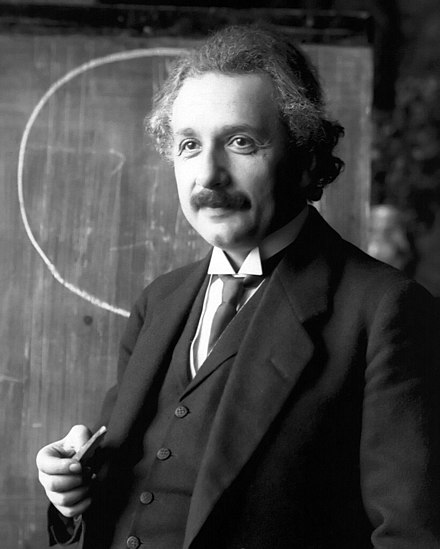
\includegraphics[width=8cm, height=8cm, keepaspectratio=true]{./content-abcd/autor1}
%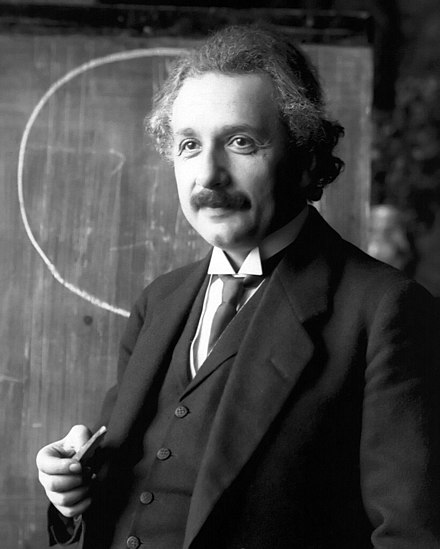
\includegraphics[width=8cm, height=8cm, keepaspectratio=true]{./content-abcd/autor1}
\end{center}

%% -- Die Referenzen werden am Ende des jeweiligen Beitrags ausgegeben
%% -- 
\begin{refsection}

%% -- Wer dies machen will
%% --
\dictum[\href{https://de.wikipedia.org/wiki/Albert_Einstein}{Albert Einstein}]{Wahnsinn ist, dasselbe immer \mbox{wieder} zu tun und andere Ergebnisse zu erwarten.}
%%
\begin{quote}
Für eine kurze Zusammenfassung
\end{quote}
%% 

%% --
\section*{Erster Hauptabschnitt}		%% 
\subsection*{Erster Unterabschnitt}		%% 
Text	
%%				
\subsection*{Zweiter Unterabschnitt}
Text
%% --
\section*{Zweiter Hauptabschnitt}		%% 
\subsection*{Erster Unterabschnitt}		%% 
%%
%% -- etc.
%% --

%% -- Literaturverzeichnis
%% --
\RaggedRight
\printbibliography
\end{refsection}

